\documentclass[10pt, compress]{beamer}
\usetheme[conference=TCV-Topic21,venue=Lausanne, date=30/05/2017, titleprogressbar, logo=RFX-logo]{Eurof}
\usepackage{listings,amsmath,multimedia, amssymb}
\usepackage{../beamerclass/tangocolors}
\usepackage{../beamerclass/rfxcolor}
% for drawing
\usepackage{pgf}
\usepackage{tikz}
\usetikzlibrary{arrows,shapes,backgrounds}
\usepackage{../beamerclass/onimage}
\usepackage[export]{adjustbox}
\usepackage{bm}
% for font
\usepackage[absolute,overlay]{textpos}
  \setlength{\TPHorizModule}{1mm}
  \setlength{\TPVertModule}{1mm}

\usepackage[style=nature,citestyle=authoryear-comp,defernumbers=true,maxnames=2,firstinits=true,
uniquename=init,backend=bibtex8,arxiv=abs,mcite]{biblatex}
\bibliography{biblio}
\renewcommand*{\bibfont}{\footnotesize}
\renewcommand*{\citesetup}{\footnotesize}
\usepackage[export]{adjustbox}
\makeatother
\mode<presentation>
\makeatletter
% add a macro that saves its argument
\newcommand{\footlineextra}[1]{\gdef\insertfootlineextra{#1}}
\newbox\footlineextrabox
% for reducing font on a single slide
\newcommand\Fontvi{\fontsize{8}{7.2}\selectfont}
\title{Topic 21: TCV experimental plan for Week 24}
\date{30 March 2017}
\author[N. Vianello,  V. Naulin]{N . Vianello and V. Naulin}
\begin{document}
\tikzstyle{every picture}+=[remember picture]
\maketitle

\begin{frame}{Taking advantage of already performed experiment}
\vspace{-1cm}
\Fontvi
  \begin{columns}
    \begin{column}{0.6\textwidth}
      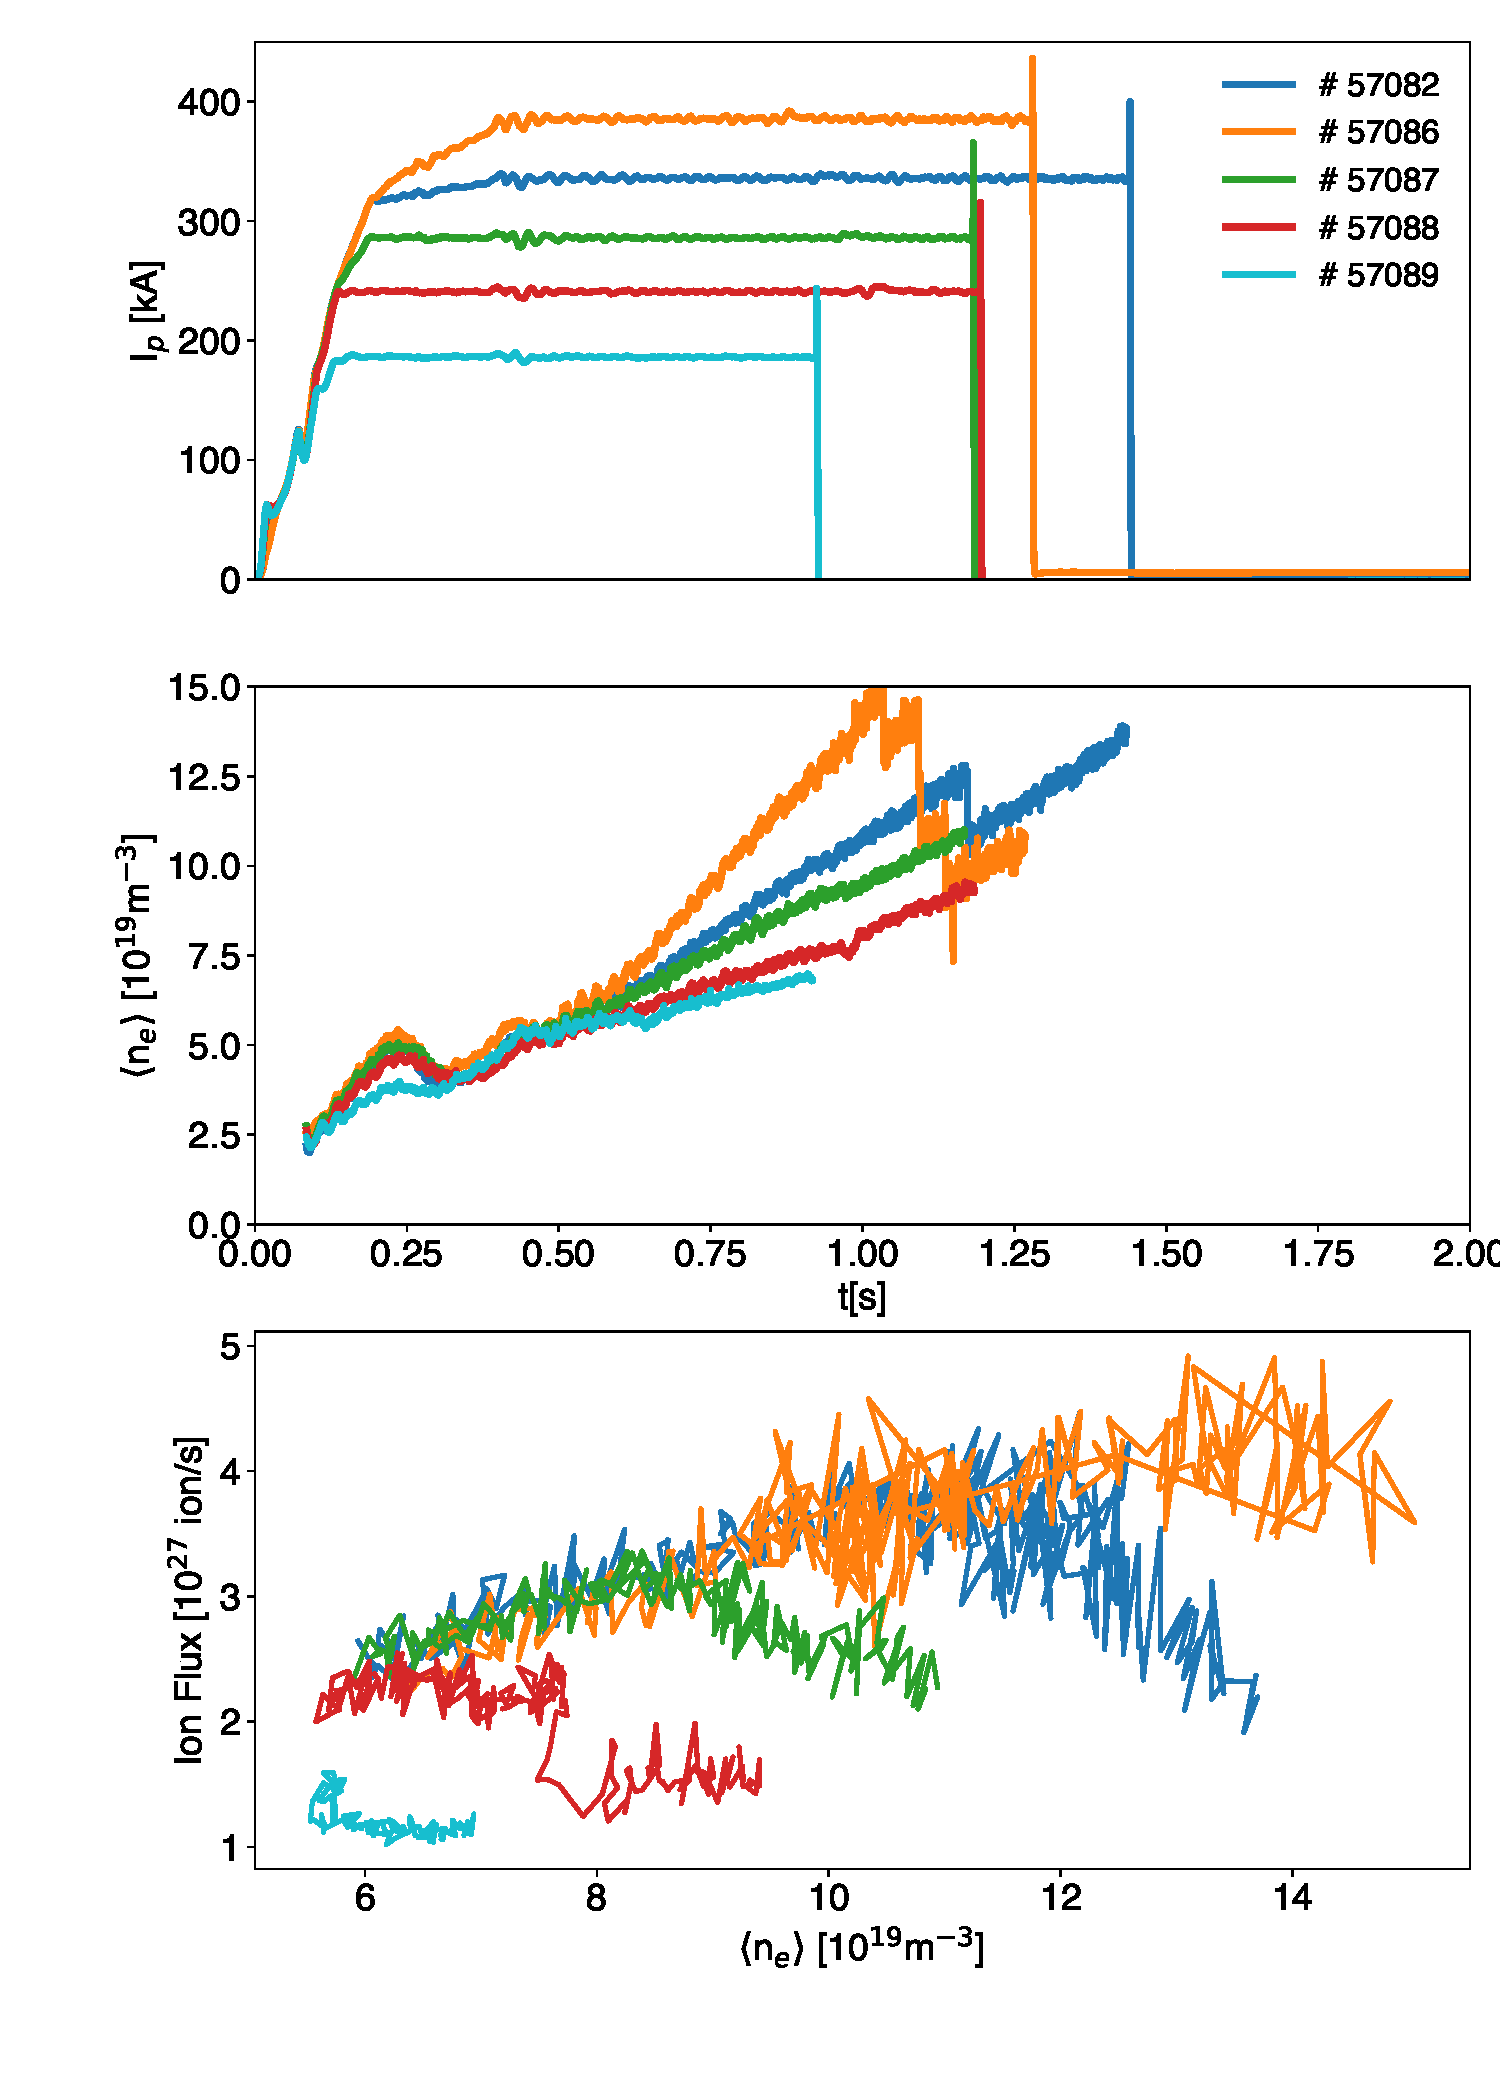
\includegraphics[width=\textwidth]{../../Experiments/TCV/analysis/pdfbox/CurrentScanTopic25}
    \end{column}
    \begin{column}{0.4\textwidth}
      \begin{itemize}
        \item Topic 25 already performed a current scan at
          constant B$_{\phi}$ but as far as I checked we don't have
          fast reciprocating probe data for all the scan \alert{To be
            confirmed by Cedric}
        \item Furthermore the density was not optimized for lower
          current, as it starts to high
      \end{itemize}
    \end{column}
  \end{columns}
\end{frame}


\begin{frame}{Proposed density ramp}
\Fontvi
  \begin{columns}
    \begin{column}{0.6\textwidth}
      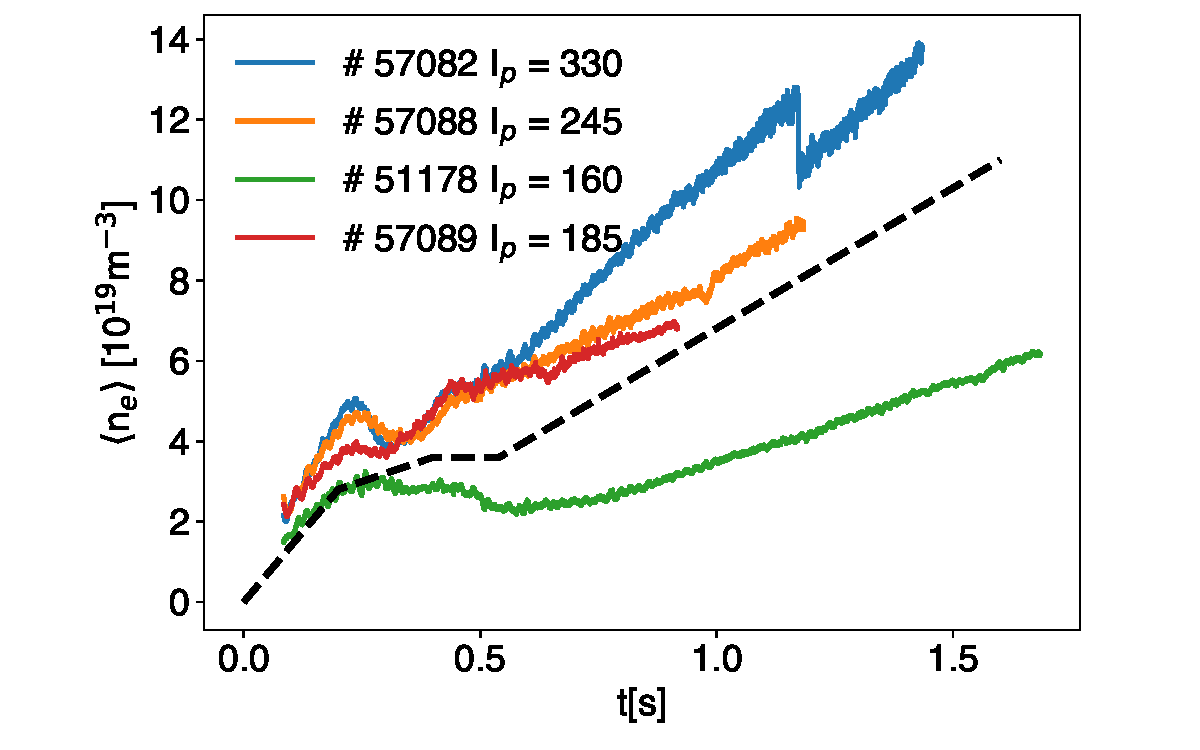
\includegraphics[width=\textwidth]{../../Experiments/TCV/analysis/pdfbox/ProposedDensityRamp}
    \end{column}
    \begin{column}{0.4\textwidth}
      \begin{itemize}
        \item The proposal is to use the same density ramp for all
          the currents as shown in dashed line. Less demanding for the
          higher current case. Risk to end with disruption for the
          lower current case
      \end{itemize}
    \end{column}
  \end{columns}
  \end{frame}

  \begin{frame}{Proposed experimental plan}
\Fontvi
    \alert{For the first week of operation we propose L-mode shots
      only. We have accomodated the low collisionality request from
      Cedric. Shots 1-3 I$_p$ scan at constant toroidal field. Shots
      1, 4 and 5 I$_p$ scan at constant q$_{95}$ to be compared with
      analogous experiments in AUG and MAST-U. Shots 6-7 Low
      collisionality scan. Shots 8-9 DN current scan: this will be
      compared directly with Mast-U which will run predominantly in DN
    configuration. Shot 10-11 Current scan in forward field to check
    the role of $\nabla\times B$ direction.}
\begin{enumerate}
\item Shape from 57088, I$_p$ = 245 kA,  Reverse B$_t$,
    density ramp from Line Average Density = 3.8e19 @ 0.5 s to 11e19 @ 1.6s,  Bt = 1.4T. Plunge @ 0.65, 1.52
\item  Repeat \# 1 with I$_p$=330 kA Bt=1.4T, same density ramp, same timing for plunges
\item  Repeat \# 1 with I$_p$=180 kA, Bt=1.4T, same density ramp, same timing for plunges
\item  Repeat \# 1 with q95=2.44 as \# 2, adjust Bt consequently (Bt = 1.02T)
\item  Repeat \# 3 with q95=2.44 as \# 2, adjust Bt consequently (Bt=0.8T)
\item  Shape and current from \# 1. Stop puffing once the divertor is
  formed to get low collisionality case. ECRH ramp from 0.9s (150
  kW--500 kW)
\item  Repeat \# 6 with intermediate density value between \# 6 and
  \#1 density at 0.65s. 
\item  Repeat density ramp of Shot \# 2 in DN configuration 
\item  Repeat density ramp of Shot \# 3 in DN configuration 
\item Repeat \# 1 in forward field
\item Repeat \# 3 in forward field
\end{enumerate}
\end{frame}
\end{document}

